\section{倾斜叠加}
\label{sec:5.2}

倾斜叠加是炮检距坐标轴的一种变换,它就像是对地震波束进行定向导引。我认为,过去
我引入术语倾斜叠加(slant stack)
只不过是把它作为以下\ref{sec:5.3}节中将述及之某种偏移方法的
一部分(Schultz与Claerbout,
1978),我确实未曾发明过倾斜叠加概念!上溯到Rieber教
授在1930年代的工作和苏联的Pa6nHKHH H.
A教授的工作,它在勘探地震学中已有一个很
长的历史了。从数学上说,倾斜叠加的概念在Radon变换(Radon,
1917)中就已奠定了基础。

倾斜叠加思想很类似于把出射角附近之数据加以组合的Snell记录道方法。Snell记录道
的思想是根据假想速度所预测出的局部时差$p=dt/dx$来选择数据,倾斜叠加却不是预测该
时差,而是进行滤波将该时差提取出来。因而,倾斜叠加不论速度是否已知均能正确地起作
用。在介质的速度是已知的时候,能够使倾斜叠加直接实现向下延拓,即使在有绕射和多次
反射的情形下出现混杂的视速度时,也能够如此。

\subsection{倾斜叠加与线性时差校正}
\label{sec:5.2.1}

在剖面或道集上寻找某种特定时差$p=dt/dx$的同相轴,相当于是对各双曲线同相轴进行
扫描以找出它们与斜率为夕之某条直线相切的地方,如利用线性时差校正将数据重新加以显
示,亦即,如将$(x,t)$平面内位于炮检距$x=g-s$和时间t上的能量转移至$(x,t')$
平面内位于炮检距x和时间$t'=t-px$
上,那末进行搜索和分析就会容易一些。这种转移过程如图
\ref{fig:slnt/lmo}所示,线性时差校正将$(x,t)$
平面内所有斜率为p的同相轴转换为$(x,t')$平面内
的“水平”同相轴,图中出现的水平计时线是为了方便于搜索和追踪测定同相轴位置。

\begin{figure}[H]
\centering
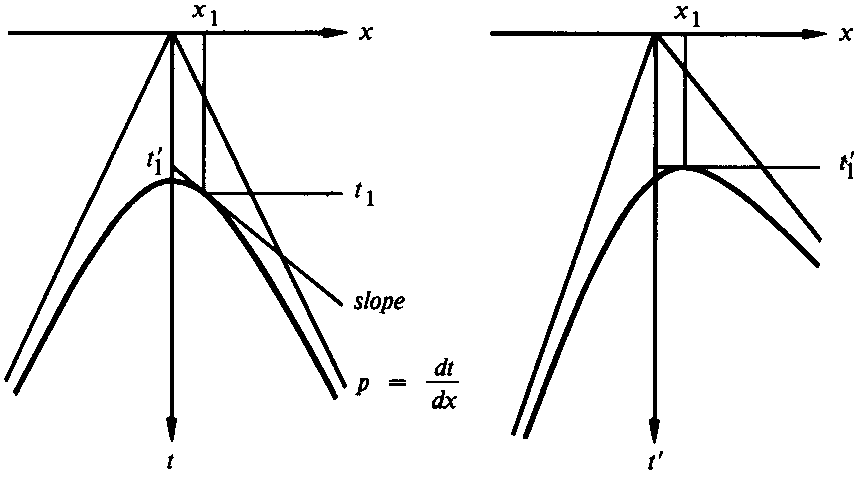
\includegraphics[width=0.65\textwidth]{slnt/lmo}
\caption[lmo]{线性时差校正将追踪识别与所构制平行直线相切之任务转
变成了给凸同相轴之顶部定位的任务}
\label{fig:slnt/lmo}
\end{figure}

在线性时差校正之后$t'=t-px$,具有Snell参量大约为p之数据中的各种组成成分就都
是沿x坐标作缓慢变化了。要提取它们,应对x坐标采用某种低通滤波处理,并对每一$t'$时间
值都如此作。低频滤波的极限情形就是提取均值,这就导致倾斜叠加的思想。

为进行倾斜叠加,要根据$t'=t-px$作线性时差校正,然后遍及x坐标求和,这样作的效
果与沿$(x,t)$平面内之倾斜直线进行求和是相同的。无论在哪种情形下,都能使整个道集
$P(x,t)$转换成作为时间广之函数的一个记录道。倾斜叠加假设遍及观测炮检距的求和可
适当代表沿炮检距坐标%的积分作用,沿炮检距坐标的倾斜积分所受到的主要影响将来自积
分路径与双曲面波至成为相切之处的区域;另一方面,在时距曲线与积分曲线相交时,对该
积分的影响就小到几乎等于零,原因就是传播之波没有零频率的成分。

波至的强度有赖于相切区域的长度,相切区长度的Fresnel定义是以半波长条件为基础
的。在速度为恒定值但有许多是平缓层的地层内,相切区之宽度因双曲线变平坦从而将随时
间而变宽,这种増宽与$\sqrt{t}$成比例,抵得上完成了一半的球面扩散校正。换言之,倾斜叠加
把我们从二维带到了一维世界,但是将三维的圆锥波阵面校正为二维的平面波还得再有个
$\sqrt{t}$。

\subsection{倾斜叠加道集是椭圆}
\label{sec:5.2.2}

数据道集的倾斜叠加产生一个以倾斜参量p为其特征的记录道,按许多p值进行倾斜叠加
处理则产生倾斜叠加道集。(具有坚实数学物理基础的读者们将会注意到,进行倾斜叠加其
实就是用Legendre变换将时距曲线加以变换,在这方面,特别条理清晰的背景读物是
H.B.Callen所著《热力学》[1960年Wiley公司出版,90页至95页])。

让我们看一下,在我们作倾斜叠加时人们熟悉的双曲线族$t^2v^2=z_j^2+x^2$会出现什么现
象。方便的办法是考虑参量形式的圆方程和双曲线方程,就是说,我们采用$z=vt\cos\theta$与 
$x=vt\sin\theta$或$x=z\tan\theta$,而不利用$t^2v^2=x^2+z^2$。令线性时差校正的方程为
\begin{equation}
\tau=t-px=t-\frac{\sin\theta}{v}x
\label{eq:ex5.2.1}
\end{equation}
利用各参量方程消去t与x
\begin{equation}
\tau=\frac{z}{v\cos\theta}-\frac{\sin\theta}{v}z\tan\theta=\frac{z}{v}\cos\theta
\label{eq:ex5.2.2}
\end{equation}
\begin{equation}
\tau=\frac{z}{v}\sqrt{1-p^2v^2}
\label{eq:ex5.2.3}
\end{equation}
取平方后得出熟悉的椭圆方程
\begin{equation}
(\frac{\tau}{z})^2+p^2=\frac{1}{v^2}
\label{eq:ex5.2.4}
\end{equation}
在各种不同反射面深度$z_j$情形下,方程\ref{eq:ex5.2.4}的图形如图\ref{fig:slnt/sstt}

\begin{figure}[H]
\centering
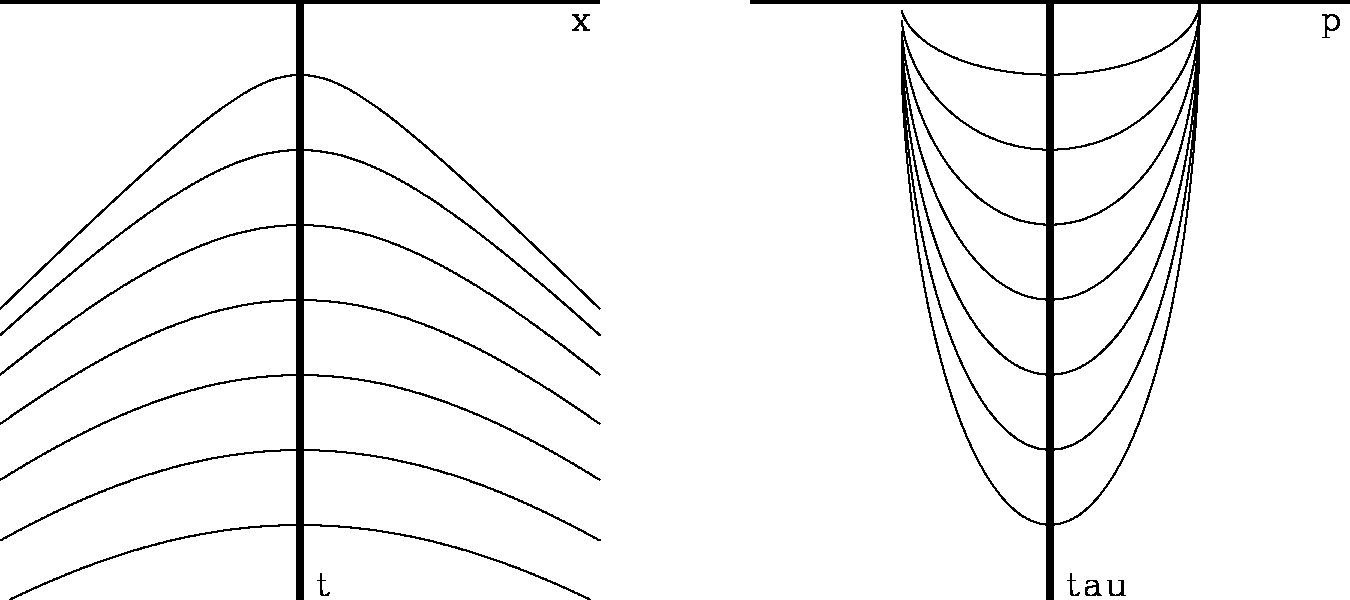
\includegraphics[width=0.65\textwidth]{slnt/sstt}
\caption[sstt]{恒定速度多层地层模型所得数据道集的时距曲线。倾斜叠加之前(左图)和之后(右图)}
\label{fig:slnt/sstt}
\end{figure}

\subsection{双层模型}
\label{sec:5.2.3}

图\ref{fig:slnt/sslayer}表示双层模型内各个波的旅行时间。正与通常情形一样,在较深地层内的速度
就较高。左图为熟悉的双曲面式的曲线,严格说,顶部的曲线是准确的双曲线,而下部曲线
仅仅是双曲面式的。通过原点的直线代表沿地表面水平方向传播的能量,下面的直线是首
波(在地震学中经常称它为折射波,不过这种名字可能引起混乱),它代表以临界角入射在
较深之地层、然后沿该分界面作水平传播的一种射线。
\begin{figure}[H]
\centering
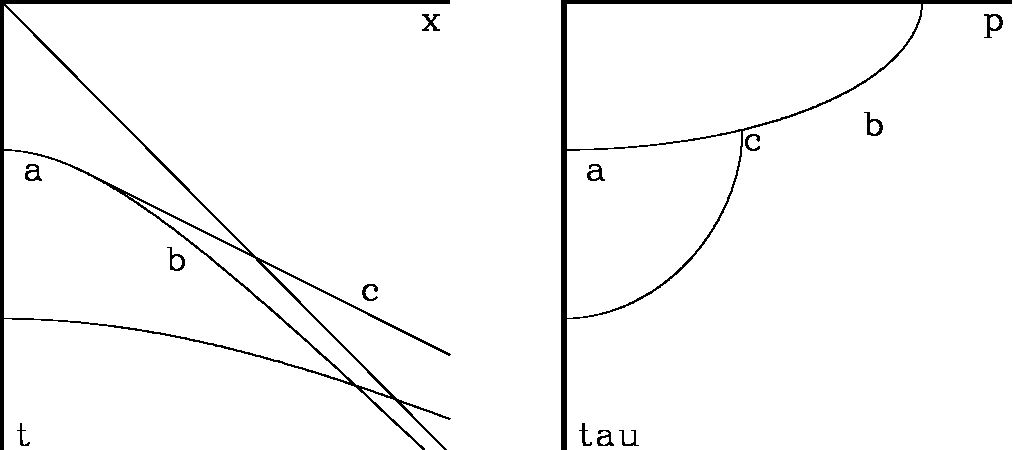
\includegraphics[width=0.65\textwidth]{slnt/sslayer}
\caption[sslayer]{识别追踪小于临界角的反射(a)、大于临界角的反射(b),及首波(c)}
\label{fig:slnt/sslayer}
\end{figure}

图\ref{fig:slnt/sslayer}的右端表示倾斜叠加之后的旅行时间曲线。注薏,在$(x,t)$空向内各曲线被
此相交,可是在$(p,\tau)$空间内它们并不彼此相交。水平坐标轴具有速度倒数之物
理量纲,每层的速度确实能够根据其旅行时间曲线按照相应椭圆上的极大值直接读出来。
首波在$(x,t)$空间内是条直线,而在$(p,\tau)$空间内则是个点,位于两个椭圆面相接触之
处。顶部的曲线在$(p,\tau)$空间内严格是一个楠圆,而下部的曲线佴仅是椭球面式的。

\subsection{根据倾斜叠加估计层速度}
\label{sec:5.2.4}

\ref{sec:1.5}节曾指出,向下延拓Snell波纯粹是个时移问题,时移量只与波的传播角度有关。例
如,关于时移的频率域方程就是
\begin{equation}
P(\omega,p,z_2)=P(\omega,p,z_1)e^{-i\frac{\omega}{r}\sqrt{1-p^2r^2}(z_2-z_1)}
\label{eq:ex5.2.5}
\end{equation}
向下延拓至第一个反射面时,我们发现第一个反射应在零时间到达。在偏移方法中,习惯的
作法是就零倾角射线来完成时间延迟,因此,延迟时间形式的向下延拓会展平第一个反射而
不改变零倾角射线。对数据进行时移使之在第一层的反射上排齐校直的过程,可用图\ref{fig:slnt/schultz}
中的第三个图形解释说明。该图的第一个图形表示速度模型,第二个图形表示地面上倾斜叠
加的结果。把第一个反射面按时间排齐校直之后,我们就得到了在第一层底部应被观测到的
数据。现在,次深曲线的是一个严格的椭圆,根据该次深的椭圆估计出次深层的速度。对所
有的深度将这种处理过程继续下去,直至处理完。这种速度估计方法是由P.Schultz
( 1982 ) 提出并试验过的。

\begin{figure}[H]
\centering
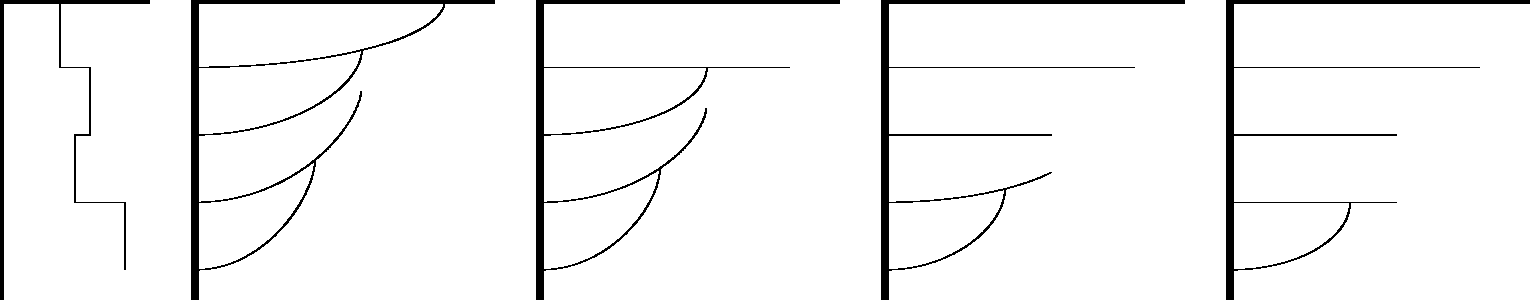
\includegraphics[width=0.65\textwidth]{slnt/schultz}
\caption[schultz]{Schultz的相继各层展平方法}
\label{fig:slnt/schultz}
\end{figure}

图\ref{fig:slnt/schultz}还解释说明了由浅层高速层引起的困难。任何较深部低速层的反射给出的是一
种不完全的椭圆,它与上面的椭圆不相联,因为它看来要延伸超出该范围。较大的p值
(图中的点状线)会丢失,因为它们被上面的高速层(低值)所阻塞限制。p的截止出现在
高速层的波趋于水平传播之处,所以,在较深的低速层底部不存在首波。

Schultz根据某个橢圆作速度沽计的方法所进行的方式是:沿各种不同速度的扫描椭圆
进行求和,然后选出具有最强叠加效果的一个速度。因此,他的方法应当不受浅层高速层的
干扰。注意下列一点是有益的,在速度随深度而连续增大的时候,速度与深度的关系曲线可
以直接从图\ref{fig:slnt/schultz}最右端的图形读出来,速度与深度的关系曲线将是联接反射各端点(极
大值)的线,亦即联接各首波的那条线。

\subsection{根据首波估计界面速度}
\label{sec:5.2.5}

根据首波确定地层速度是地震学中的一个古老问题了
。在有可能的地方根据首波测定速
度是指在特定的深度上进行测定---分界面深度---所以,它具有甚至比层速度(两个反射
之间的深度间隔上的速度)还要好的深度分辨能力。

按传统的作法,首波速度分析涉及到识别追踪旅行时间。旅行时间很难在受干扰资料中
识別出来。Clayton与McMechan (1981)曾介绍过一种建立在波场本身基础上的、而不是
在追踪旅行时间基础上的新方法,他们解决首波速度分析问题就同波动方程偏移解决反射问
题一样。

与那类从剖面上的反向散射首波获取速度信息(见\ref{sec:3.5}节)的方法相同的思想,可以应
用于共中心点道集中的普通首波。在道集中,你可得到在向下延拓将能量聚焦到零炮检距的剖
面上所没有的额外信息。聚焦点可不是一个平凡的毫无特色的点。取一段没有反射而仅由一
个首波所组成的原始数据,向下延拓后在零炮检距上产生一聚焦点,该聚焦点是把具有和原
始未聚焦首波一样的时差$dt/dh$之零散能量集中起来而得到的结果。按所有可能的取向将各
聚集点相加起来(倾斜叠加),
从而把数据$u(h,\tau)$变换至倾角空间、比方说变换为$\bar{u}(p,\tau)$。在$(p,\tau)$
平面上地震能量已经集中的地方求出旅行时间深度$\tau$处地层的速度,该速度可
直接由$v(\tau)=1/p(\tau)$得出。已知$v(\tau)$,很容易就能求出$v(z)$。或者,整个计算过程也可以直接
按深度z来实现而不按旅行时间深度$\tau$来完成。

Clayton与McMechan实际
是按相反的顺序来完成向下延拓和倾斜叠加的,他们首先是倾斜
叠加,然后再向下延拓的。在原理上,这些赴理过程不论按什么
顺序完成都行。要记住,我们是否成功是脱离不开正确的地层速
度的,进行倾斜叠加倒是不必
依靠地层速度,但是向下延拓却得依靠正确
速度。倾斜叠加仅需实现一次,如果它是首先
作的话。这就是为什么Clayton和McMechan按那种顺序方式作它的原因。图5.
2-5和图5.2 -6所示是他们的实例之一。

将Clayton与McMechan的方法同Schultz的方法比较一下。Schultz是用一种对椭
圆较大p值部分很敏感的方法将反射展平,
Clayton与McMechan则只着眼于椭圆的最大
p值部分。Schultz方法的好处是:一种以反射为
基础的方法是不受高速层干扰时,但是缺点是
要求在向下进行处理之际就得作出判断决定。
Clayton与MeMechan则是把一个信息平面提
供给解释者,由解释者从这个平面中去选择速度。Clayton与MaMechan的速度空间是数据
的一个线性可逆函数,\ref{sec:5.4}节将要阐述从反射数据(不是首波)至速度空间的线性可逆变换。

\begin{figure}[H]
\centering
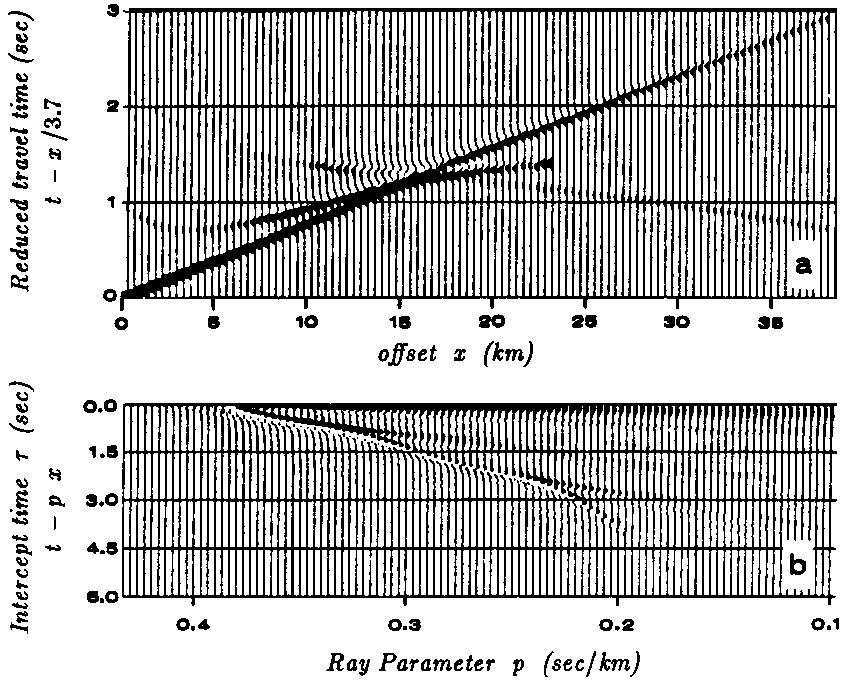
\includegraphics[width=0.65\textwidth]{slnt/sshead}
\caption[sshead]{上图(a)是包含有一合成首波的剖面(以线性时差校正方式显示)
利用倾斜叠加将数据变换如图(b)的下半部分所示。这个已经过倾斜叠加的波场(b)的向下
延拓结果如图\ref{fig:slnt/sshead2}所示(Clayton与McMechan)}
\label{fig:slnt/sshead}
\end{figure}

\begin{figure}[H]
\centering
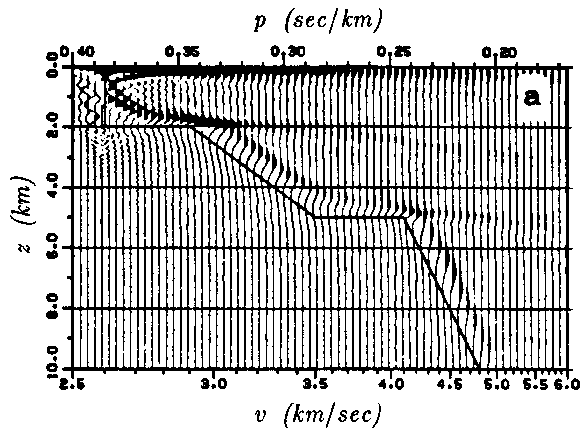
\includegraphics[width=0.65\textwidth]{slnt/sshead2}
\caption[sshead2]{以正确的速度与深度关系函数(图中实线)对图\ref{fig:slnt/sshead}(b)
中的倾斜叠加波场进行向下延拓的结果}
\label{fig:slnt/sshead2}
\end{figure}

\subsection{倾斜叠加与Fourier变换}
\label{sec:5.2.6}

设$u(x,t)$为波场。在数学上,波场的倾斜叠加$\bar{u}(p,\tau)$被定义为:
\begin{equation}
\bar{u}(p,\tau)=\int u(x,\tau+px)dx
\label{eq:ex5.2.6}
\end{equation}
式\ref{eq:ex5.2.6}中,按x进行的积分是在$\tau$值恒定时完成的,积分路程就是$(x,t)$平面内的某条
倾斜直线。

在Fourier空间内很容易表示倾斜叠加。波场$u(x,
t)$的二维Fourier变换之定义为:
\begin{equation}
U(k,\omega)=\\int e^{i\omega t-ikx}u(x,t)dxdt
\label{eq:ex5.2.7}
\end{equation}
回想一下Fourier空间内的Snell参量定义$p=k/\omega$,利用它从式\ref{eq:ex5.2.7}
的二维Fourier变换中消去k
\begin{equation}
U(\omega p,\omega)=\\int e^{i\omega(t-px)}u(x,t)dxdt
\label{eq:ex5.2.8}
\end{equation}
将积分变量由t改变为$\tau=t-px$
\begin{equation}
U(\omega p,\omega)=\int e^{i\omega\tau[\int u(x,\tau+px)dx]}d\tau
\label{eq:ex5.2.9}
\end{equation}
把式\ref{eq:ex5.2.6}定义代入式\ref{eq:ex5.2.9},得
\begin{equation}
U(\omega p,\omega)=\int e^{i\omega\tau} \bar{u}(p,\tau) d\tau
\label{eq:ex5.2.10}
\end{equation}
把$U(\omega p,\omega)$看作是$\omega$的一维函数,该$\omega$是从$(k,\omega)$平面沿直线$k=\omega p$
提取的。

式\ref{eq:ex5.2.10}的Fourier逆变换为
\begin{equation}
\bar{u}(p,\tau)=\int e^{-i\omega \tau}U(\omega p,\omega)d\omega
\label{eq:ex5.2.11}
\end{equation}

式\ref{eq:ex5.2.11}的结果阐明可以用Fourier域运算来形成倾斜叠加。首先,你把$u(x,t)$变换为
$U(k,\omega)$;然后,从$U(k,\omega)$提取出$U(\omega p,\omega)$;最后,从$\omega$域反变换至$\tau$域并
对所有感兴趣的p值重复上述过程。

从$U(k,\omega)$得出$U(\omega p,\omega)$看似很容易,但这其实是很难作的部分。直线$k=\omega p$以不
会恰好通过所有的网格点(除非$p=\Delta t/\Delta x$),所以必须作某种内插。正如我们由Stolt偏移
的计算假象所已经知道的,不应该按因果性条佇要求来作频率域内插。有关内插的意见可参
阅\ref{sec:4.5}节。

实际应用时,既可采用式\ref{eq:ex5.2.6}也可采用式\ref{eq:ex5.2.11}。应用式\ref{eq:ex5.2.6}时,你能
对截断效应和假频现象进行较好的控制;在处理大型数据组资料的情形下,则采用式\ref{eq:ex5.2.11}就能使计算非常快速。

\subsection{逆倾斜叠加}
\label{sec:5.2.7}

医学成像中的Tomography
(层析成像分析)建立在与逆倾斜叠加是相同的数学基础
上。筒单地陈述,二维Tomography或逆倾斜叠加就是在已知某个函数的线积分的条件下重
建该函数。遵照二维Fourier积分的定义就能得出逆倾斜叠加的公式为
\begin{equation}
u(x,t)=\int e^{-i\omega t[\int e^{ikx}U(k,\omega)dk]d\omega}
\label{eq:ex5.2.12}
\end{equation}
将$k=\omega p$和$dk=\omega dp$代入式\ref{eq:ex5.2.12}。注意,当$\omega$为负时,对dp的积分要从正积到负而不
是相反。为保持从负积至正之常规习惯意义上的积分方法,现在引入绝对值$\mid\omega\mid$。(更一般
性地说,改变体积分的变量要引入变换的Jacobi行列式)。因而
\begin{equation}
u(x,t)=\int e^{-i\omega t}[\int e^{i\omega px}U(\omega p,\omega)\mid\omega\mid dp]d\omega
\label{eq:ex5.2.13}
\end{equation}
\begin{equation}
u(x,t)=\int\{\int e^{-i\omega t}[U(\omega p,\omega) e^{i\omega px}\mid\omega\mid ]d\omega\}dp
\label{eq:ex5.2.14}
\end{equation}
注意到在式\ref{eq:ex5.2.14}的花括号$\{\}$内包含着的是三个频率函数之乘积的Fourier逆变换,频
率$\omega$域内三个函数之乘积在时间域内就是某种褶积。这三个函数中,第一个是$U(\omega p,\omega)$,
按式\ref{eq:ex5.2.11}的定义,它就是倾斜叠加的Fourier变换;第二个是延迟算子那就是
位于时刻的脉冲时间函数;第三个是一种$\mid \omega \mid$滤波器,该$\mid \omega \mid$滤波称作rho滤波,由于
rho滤波与p值无关,所以我们能把它从对p的积分中分离出来。设以符号*表示褶积,引入
延迟px作为自变量移位,我们最终就得到一直为我们所追求的逆倾斜叠加方程:
\begin{equation}
u(x,t)=rho(t)*\int \bar{u}(p,t-px)dp
\label{eq:ex5.2.15}
\end{equation}
稀奇的是,倾斜叠加运算\ref{eq:ex5.2.6}的逆过程竟基本上是改变符号进行另一种倾斜叠加的运算\ref{eq:ex5.2.15}。

\subsection{平面波叠合}
\label{sec:5.2.8}

式\ref{eq:ex5.2.15}可以简单解释为平面波叠合。为将这点说清楚,我们首先依靠下列一种定
义来处置rho滤波
\begin{equation}
\tilde{u}(p,\tau)=rho(\tau)*\bar{u}(p,\tau)
\label{eq:ex5.2.16}
\end{equation}
将会看出式\ref{eq:ex5.2.16}不仅仅只是一种定义式,我们还认识到可以把$\tilde{u}(p,\tau)$
解释为是平面波谱。把定义式\ref{eq:ex5.2.16}代入式\ref{eq:ex5.2.15}与式\ref{eq:ex5.2.6}二者中去,得出另一对变换:
\begin{equation}
u(x,t)=\int \tilde{u}(p,t-px)dp
\label{eq:ex5.2.17}
\end{equation}
\begin{equation}
\tilde{u}(p,\tau)=rho(\tau)*\int u(x,\tau+px)dx
\label{eq:ex5.2.18}
\end{equation}

为证实$\tilde{u}(p,\tau)$能够被解释为平面波谱,我们令$\tilde{u}(p,\tau)$为脉冲函数$\delta(p-p_0)
\delta(\tau-\tau_0$并代入式\ref{eq:ex5.2.17},正如所料,所得结果$u(x,t)=\delta(t-p_0x-\tau_0)$正是一
个脉冲平面波。

\subsection{反射系数---球面波与平面皮情形的对比}
\label{sec:5.2.9}

你在野外剖面上看到的反射波振幅是受许多事情影响的。假设对波的球面发散、通过各
层时的透过系数、层内多次反射等等的影晌均可作校正,留下来的就剩球面波反射系数了。
球面波反射强度同《地球物理数据处理基础》一书中所计算出的或用Zeoppritz(
1919)方
程计算出的平面波反射系数并不是相同的一回事。反射系数强度的理论分析总是以Fourier
分析为基础。方程\ref{eq:ex5.2.17}与\ref{eq:ex5.2.18}提供了平面波反射系数与柱面波反射系数之间
的联系,至于如何再由柱面波情形通向球面波情形,请看\ref{sec:3.5}节中关于切除与加权那一小节
的讨论\footnote{
这一节的中心意思是说:采用Fourier分析方法进行反射系数分析,只适用于一维平面波情形;利用式\ref{eq:ex5.2.17}
与式\ref{eq:ex5.2.18}这一对正、反倾斜叠加变换处理,就可以进行二维柱面波情形下的反射系数分析;在此基础之上,采用
\ref{sec:3.5}节所述按炮检距进行加权的办法,则可进一步作三维球面狡情形下的反射系数分析。---译者
}。

\subsection{rho滤波}
\label{sec:5.2.10}

在实际工作中,往往忽略rho滤波,因为可以把它合并到总的数据记录与处理过程中其余
的滤波效果中去。然而。rho滤波不是微不足道的,倾斜叠加中的积分运算会增强低频成分,
而rho滤波则把它们座制到使之保持适当水平。现在让我们对这种滤波作一番检查。滤
波的谱同时间导数的谱是相同的,但是它们的时间函数却非常不同。时间导数的有限差分
表现形式很短,时间延续长度仅为$\Delta t$;因为绝对值函数有尖锐变化,rho滤波却具有很长的
时间延续。Hilbert积分核$-1/t$的Fourier变换是$isgn(\omega)$,要注意,$\mid
\omega\mid = (-i\omega)\times i sgn(\omega)$,在时间域内这个关系式意味着应有
$\frac{d}{dt}(-\frac{1}{t})=\frac{1}{t^2}$,因此$rho(t)=\frac{1}{t^2}$。

还有一种不同的观点是:应将$rho$滤波划分为两部分,一半参与正向倾斜叠加,另一半
则参与反向倾斜叠加,这时进行倾斜叠加将不会使数据的功率谱引起变化。一种有趣的划分
$\mid \omega\mid$的方式是令$\mid\omega\mid=\sqrt{-i\omega}\sqrt{i\omega}$,在
\ref{sec:4.6}节中已指出过$\sqrt{-i\omega}$是相应于因果性时间函
数,而是相应于反因果性时间函数。在Phinney等人的论文(Phinney et
al.,1981)中可找到关于倾斜叠加的更多细节。

实际上,倾斜叠加并不像二维Fourier变换那样地完全可逆,所以往往要采用各种的递
归和最优化技术。








